\subsection{Controller Subsystem}
\label{sec:controller_subsystem}
% Why the MCU connects to the internet
In order for our system to be as self and power efficient as
possible from an end-user perspective, it was determined that our product may an internet connection to allow the user to view measurements and change settings. To make the process of operating our product as hands-off as possible to end-users, the microcontroller can connect to the user's home WiFi network to post results and possibly access APIs. Bluetooth, Zigbee, Thread,
and other short-range 2.4 GHz communication protocols were disfavored over WiFi, as we predict most users will not have a device dedicated to connecting our product via such protocols. Long range (LoRa) protocols were deemed unncessary, as the intended placement of our product is outside, near or next to the user's home. We do not expect our product to produce or receive large amounts of data, so the decreased bandwidth of a WiFi-enabled product being beyond the outdoor walls of a building is not a significant drawback to our application. A wired connection (802.3/Ethernet) was deemed too invasive to the end-user. It is expected that most, if not all, end-users have a wireless access point and internet access. Thus, connection via the 802.11/WiFi standard was a natural choice for our use case.

% How the MCU connects to the internet (local network, LAN -> NAT -> WAN,
% TCP stack)
\paragraph{CC3220 Overview}
The Texas Instruments CC3220-series (hence referred to as the "CC3220", the "MCU", or the "microcontroller") of microcontrollers are WiFi-enabled chips with an ARM Cortex-M4 central processor and a WiFi network processor, along with many useful peripherals and power management modules. This series of processors is delivered alongside a software  evelopment kit (SDK) provided by Texas Instruments to ease the development of Internet-of-Things (IoT) applications.

\begin{figure}[H]
    \caption{Control subsystem block diagram}
    \label{fig:control-block-diagram}
    \centering
    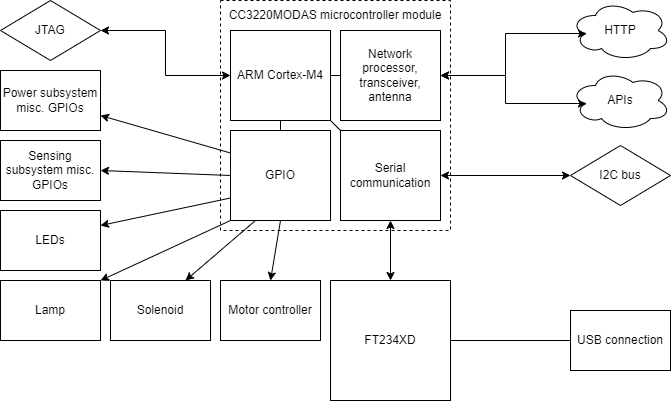
\includegraphics[width=0.9\textwidth]{images/control-block-diagram.png}
\end{figure}

The CC3220's WiFi network processor (NWP) supports the following
standards/features useful to our development
(see \autoref{cc3220_network_subsystem}):
\begin{itemize}
    \item WiFi standards: 802.11b/g/n
    \item WiFi security: WEP, WPA/WPA2 PSK, WPA2 enterprise, WPA3 personal,
    WPA3 enterprise
    \item WiFi provisioning: SmartConfig, WPS2
    \item IP protocols: IPv4, IPv6
    \item IP addressing: static IP, DHCPv4, DHCPv6
    \item Transport: UDP, TCP, RAW
    \item Host interface: UART, SPI
\end{itemize}
The CC3220's networking subsystem is identical to the CC3220's, and is further detailed in \autoref{cc3220_network_subsystem}.
\begin{figure}[H]
    \caption{CC3220 networking subsystem \cite{swru455m}}
    \label{cc3220_network_subsystem}
    \centering
    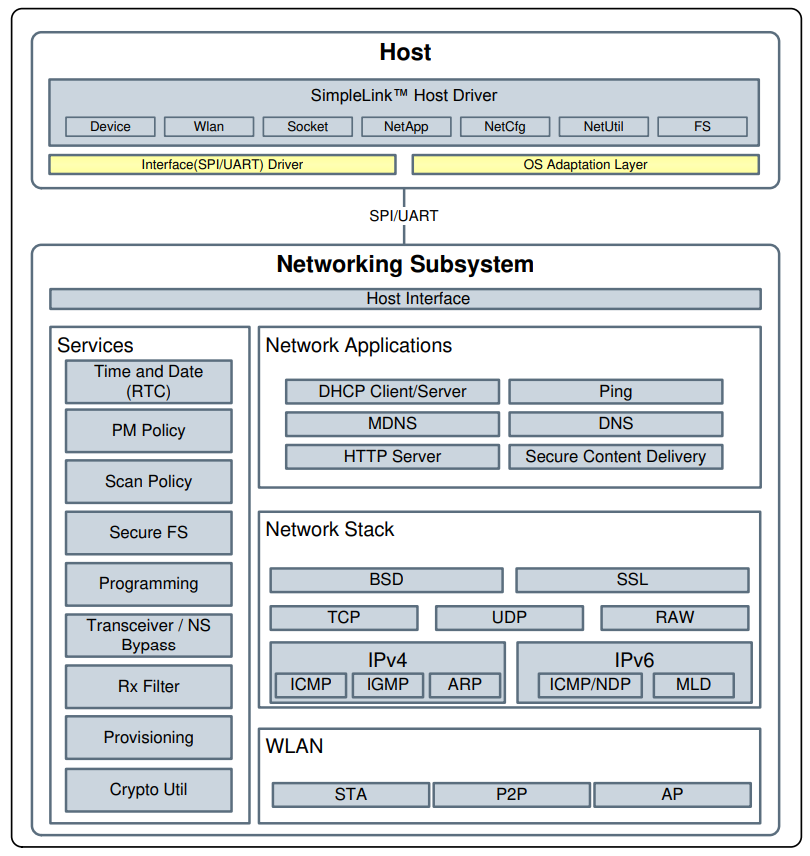
\includegraphics[width=0.75\textwidth]{images/cc3220_network_subsystem.png}
\end{figure}
\paragraph{Connection}
On startup, our microcontroller operates in AP mode and broadcasts an SSID for the user to connect to. They can then provision the NWP to connect to their own WLAN in station mode,or they can provision it via SmartConfig. The system can receive an IPv4 address via DHCP, or it can be statically assigned.

% Any over-the-air updates?
\paragraph{Over-the-Air Updates}
The microcontroller does not support over-the-air updates.

\paragraph{Startup} Upon startup, the system initializes the systems' threads and starts the RTOS. The main thread initializes these peripherals within 30 seconds of startup: GPIO, ADC, UART, I2C, NWP. It initializes the ADC and moves the motor to its maximum position. The power thread initializes the charge controller. The water thread initializes the water solenoid. The web thread initializes the HTTP server on the NWP.

\paragraph{Shutdown} Expected or unexpected shutdowns are treated the same, and are safe to the user and the system. Code stops being executed immediately, and the system will start up normally the next time it is powered on.

\paragraph{Software Logic Flow} The control subsystem software follows the logic flow detailed in \autoref{fig:logic-flow}.

\begin{figure}[H]
    \caption{Control subsystem logic flow diagram}
    \label{fig:logic-flow}
    \centering
    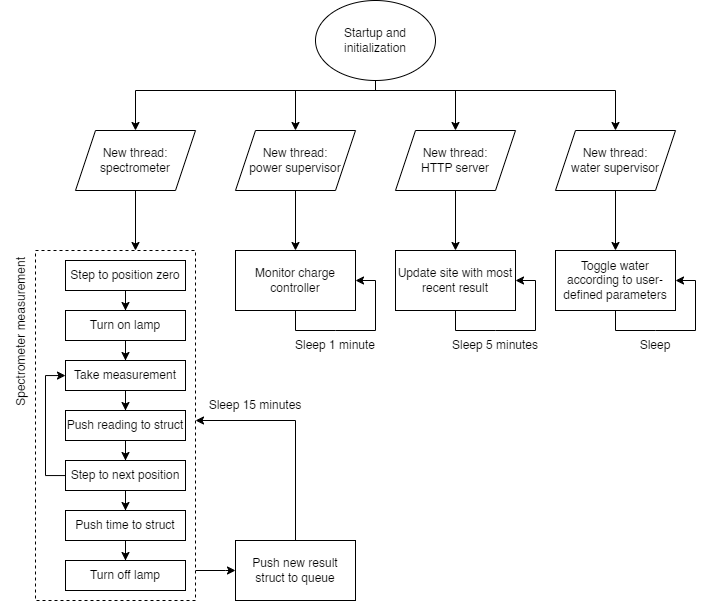
\includegraphics[width=0.9\textwidth]{images/logic-flow.png}
\end{figure}

\paragraph{Spectrometer} To perform a spectrometer measurement, the system steps the motor to its maximum position (spectral position zero). The system turns on the lamp, and takes readings from both channels of the ADC. The system passes the reading to the struct its created, and steps to the next position. The system takes a reading from both channels, and steps to the next position. It repeats this process for all spectral positions, and saves the current time to the struct afterwards. It turns off the lamp, and pushes the struct to the Sensing class's queue. The system sleeps for 15 minutes and repeats the measurement process again.

\paragraph{Power Supervisor} Because the battery and charge controller weren't implemented, this thread is empty.

\paragraph{HTTP server} This thread is managed automatically by the NWP. Because publishing to the web page was not implemented, the server home page displays "Hello, World!" and the system date and time. The network settings can be accessed and changed.

\paragraph{Networking} The system can connect to the user's 2.4 GHz-based wireless network. The network must adhere to the standards of 802.11b, g, or n. The system receives an IPv4 address assigned by network DHCP, or the user can statically assign a local IPv4 address.

% Parameters for connection and how often it tries
\paragraph{Weather API Implementation}
As a stretch goal, the user will be able to configure the MCU in Station mode to allow it to connect to the user's home WLAN's SSID as a client. The user would still be able to access the MCU's web portal and see the same information as they had before. In addition, the MCU would be able to access an API to receive weather information and inform the user of recommended actions pertaining to their garden bed (e.g. if the system determines there will be freezing temperatures overnight, it may suggest to the user to cover the garden bed with a sheet or towel).

\paragraph{Water Supervisor} This thread toggles the water on for 10 seconds every 24 hours.

% Will program in C++. Any libraries, multithreading?
% Singleton Pattern Thread for scheduling tasks
\paragraph{C++ Structure}
The C++14 standard library as implemented by Texas Instruments' ARM compiler were used, as well as POSIX and the Texas Instruments SimpleLink CC32xx SDK.

\paragraph{Singleton-Meyers Pattern}
The Meyers' Singleton design pattern was used for most of the classes found in our project repository (e.g. for our water solenoid class as seen in \ref{fig:singleton_implementation}). Because our team is using a RTOS with a scheduler and threads, we are using that to our advantage to divide and schedule tasks for the different submodules of our project. However, one problem our team took into consideration is that there is was only one physical instance of each submodule. The normal Singleton pattern traditionally has been used when one wants only one instance of a class initialized at any one point, but they are not thread-safe. One variation of this pattern is the Meyers' Singleton, which guarantees that only one instance of a type is available at any time. Initialization of this pattern is thread-safe, and locks can be used to ensure thread safety when accessing members of the class. This is accomplished by using a static local variable inside a static member function to hold a single instance of the class. The Meyers' Singleton takes advantage of the fact that the initialization of static local variables inside functions is guaranteed to be thread-safe. The Meyers' Singleton disallows copying and moving of the class, and makes member constructors and destructors private.

% Code style
\lstdefinestyle{mystyle}{
    basicstyle=\ttfamily\footnotesize,
    breakatwhitespace=false,         
    breaklines=true,                 
    captionpos=b,                    
    keepspaces=true,                 
    numbers=left,                    
    numbersep=-15pt,                  
    showspaces=false,                
    showstringspaces=false,
    showtabs=false,                  
    tabsize=2
}
\lstset{style=mystyle}

\begin{figure}
    \centering
    \label{fig:singleton_implementation}
    \caption{An example of the Meyers' Singleton pattern implementation within the project.}
\begin{lstlisting}[language=C++]
    class Water { 
        public:
            static Water& instance();

            // Disallow copying
            Water& operator = (const Water&) = delete;
            Water(const Water&) = delete;

            // Disallow moving
            Water& operator = (Water&&) = delete;
            Water(Water&&) = delete;

            // Class functions
        
        private:
            Water();
            ~Water();

            // Class variables
    };
\end{lstlisting}
\end{figure}

% Classes and class diagram
\paragraph{Classes}
There is a few classes defined in the MCU's programming, detailed
in \autoref{classes_uml}. Classes are laid out in the header file
according to the definitions given in the UML diagram.
\begin{figure}[H]
    \caption{UML diagram of the classes used}
    \label{classes_uml}
    \centering
    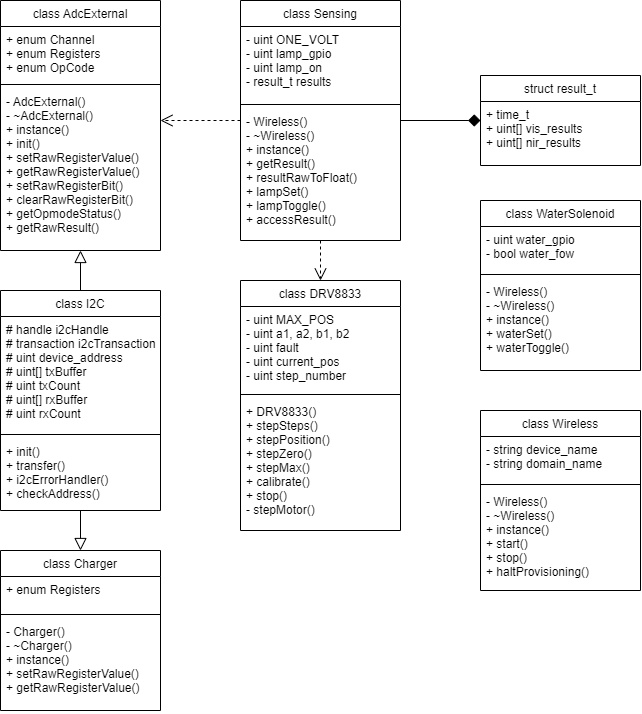
\includegraphics[width=\textwidth]{images/classes_uml_new.png}
\end{figure}

% File organization (main, header files, other source files, etc.)
\paragraph{File Organization}
Classes, macros, functions, and variables are defined/prototyped to the
extent required in headers file to be named according to their subsystem with the header file extension \texttt{.hh}. These
classes, functions, and variables are further defined in a seperate
source file named \texttt{*.cpp} as needed. The \texttt{main()}
function and the remaining classes, macros, functions, and variables,
required are located in \texttt{main\_tirtos.cpp}.

% How the MCU gets data from sensors (ADC)
\paragraph{Data} As well as being able to see and configure the network settings of the product, the user is able to see data relating to the OH-levels and common plant nutrient levels as determined by the spectral analysis of the product. For one measurement, our team needs to store 16 bits of data per position from 130 unique positions, per sensor.
\begin{equation}
    \frac{16\,\mathrm{b}}{8\,\mathrm{b/B}}\times 130\,\mathrm{positions} \times 2\,\mathrm{sensors} = 520\,\mathrm{B}
\end{equation}
With 8 Mb of the 32 Mb (1 MiB of the 4 MiB) shared serial flash dedicated to storing results, this allows us to store 2016 measurements.
\begin{equation}
    \frac{1\,\mathrm{MiB}}{520\,\mathrm{B/measurement}} = 2016\,\mathrm{measurements}
\end{equation}
Stretching out measurements to be recorded every 15 minutes, this allows a user to see individual measurements stretching back exactly three weeks.
\begin{equation}
    2016\,\mathrm{measurements} \times \frac{1\,\mathrm{measurement}}{15\,\mathrm{min}} = 30240\,\mathrm{min} 
\end{equation}
As a stretch goal these measurements can be aggregated and analyzed, and allow us to serve trends and predictions to the user.

% How MCU sends data to servos
\paragraph{Motor Controller}
Four GPIO lines are used to control the stepper motor holding the sensing PCB (which includes the photodiodes, op-amp circuitry, ADC, motor controller, and connector). Depending on the digital values passed to the motor controller, the motor controller is able to control the movement direction and speed. Our team found that using the SimpleLink SDK's high-level hardware abstraction layer (HAL) provides too long of a delay when changing values in the four GPIO lines. Nanosecond-levels of delay were needed, rather than the microsecond levels of delay our team was seeing. Instead of using highly-abstracted APIs for control of the motor, our team got as close to hardware as is possible with C/C++ and used TI's driverlib driver library specifically for the CC3220. Instead of a simple GPIO number being passed to the function, our team had to determine the GPIO port and port-specific pin of each input of our motor controller. The driverlib function checks the port for correctness, and then performs a system call to write a value directly to memory (in our case, the address of the GPIO port). Using driverlib also allows us to bit stuff our GPIO pins if they are located on the same port---in our second iteration of the board, the motor controller GPIOs were relocated to the same GPIO port and bitmasks used so we can change all four GPIO pins with one driverlib write function. This allows us to toggle a single GPIO pin within a period of 350 ns (seen in \ref{fig:gpio_toggle_driverlib}). With a speed of 80 MHz in active mode, this would mean we're able to write to GPIO in only 28 processor cycles.
\begin{equation}
    350\,\mathrm{ns} \times (80\times10^6\mathrm{cycles/s}) = 28\,\mathrm{cycles}
\end{equation}
This is a huge accomplishment for our team, especially with a program written in C++ and utilizing HAL.

\begin{figure}[H]
    \centering
    \label{fig:gpio_toggle_driverlib}
    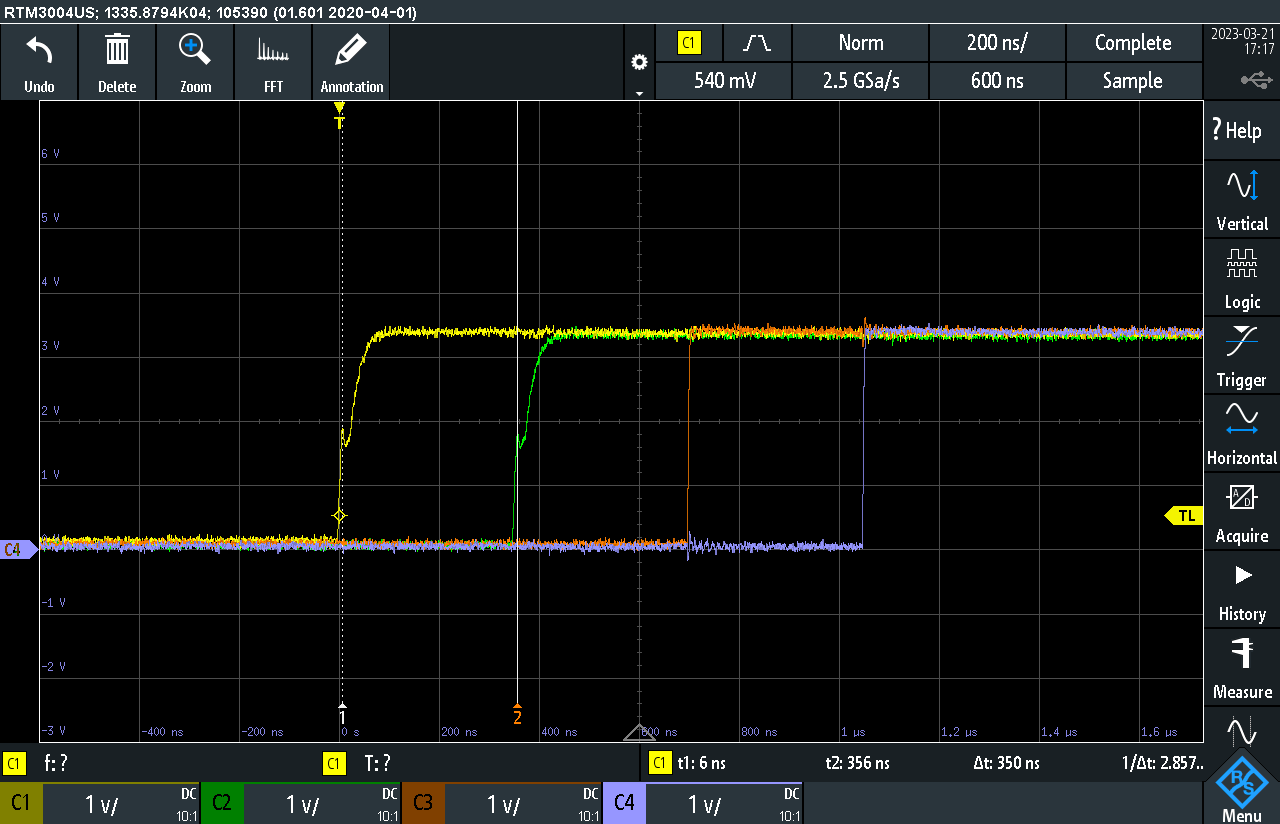
\includegraphics[width=\linewidth]{images/gpio_toggle_driverlib.jpg}
    \caption{Toggling GPIO using driverlib results in a very short (350 ns) delay.}
\end{figure}
To drive a DC motor we similarly needed a device to separate the digital logic from the back emf of the motor. This is done through the use of the motor driver. The timing of the signals is the most important part as the driver is just using the current and voltage source designed specifically for the motor in the timings given by the input pins. Wrong timing leads to the ability to skip tests leading to indeterministic behavior. The issue is the the CC32xx SDK abstracts away a lot of the fine tunability of setting hardware registers. To resolve this, the team used the specific board's hardware driver implementation to set the output on the pins with a delay of only 28 cycles.

% What kind of development model?
\paragraph{Development Model}
An Agile development model was used. Code reviews were performed on
an as-needed basis by the team.
\begin{figure}[H]
    \caption{UML diagram of the subsystem's development methodology}
    \label{mcu_agile_uml}
    \centering
    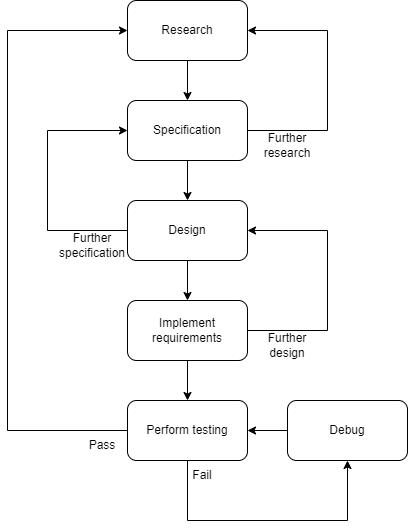
\includegraphics[width=0.65\textwidth]{images/mcu_agile_uml.png}
\end{figure}

% IDE and Git
\paragraph{IDE and Git}
Texas Instruments Code Composer Studio v12 were used to program,
compile (via TI ARM compiler v20), and debug the C++-based project. GitHub
was used as a repository for the project, using Git for version
control.

% Power
\paragraph{Power}
The MCU is connected to power from the power subsystem detailed in \autoref{sec:power_subsystem}, and receives 3.3 V, 5 V, and 12 V. 3.3 V is fed to the integrated DC/DC converter on the CC3220, as well as passed through to the sensing subsystem. 5 V is passed on to the sensing subsystem for the motor and motor controller. 12 V is passed to the Darlington pairs to control the lamp and water solenoid.

% LEDs
\paragraph{LEDs} The system is able to make use of its onboard LEDs for notifying the user or developers of system states. When the system is in active mode, the green LED shall be solidly illuminated. When the system is in low power mode, the green LED shall flash 1 time for a period of 0.5 seconds, every 2 seconds. When the system is in critical power mode, the red LED shall flash 2 times for a period of 0.5 seconds per flash, seperated by 1 second between each flash, every 30 seconds. When the system is in shutdown mode, no LEDs shall be active. When the system is starting up, the green and red LED shall be solidly illuminated until the startup sequence is completed and the system transitions into a different power mode. The yellow LED shall solidly illuminate while receiving data through the RF antenna for
the duration of the reception. The yellow LED shall blink 1 time every 0.2 seconds for a period of 0.1 second while transmitting data through the RF antenna for the duration of the transmission.

\begin{table}
	\centering
	\begin{tabularx}{\textwidth}
		{
			| >{\raggedright\arraybackslash}X
			| >{\raggedright\arraybackslash}X
			| >{\raggedright\arraybackslash}X
			| >{\raggedright\arraybackslash}X
			|
		}
		\caption{MCU LED operation}
		\label{table:mcu_leds} \\
		\hline
		\textbf{Power Mode} & \textbf{Red LED} & \textbf{Yellow LED} & \textbf{Green LED} \\
		\hline
        \textbf{Active} & Not active & RX: Solidly illuminated, TX: 1 flash of 0.1 s, every 0.2 s & Solidly illuminated \\
        \hline
        \textbf{Low} & Not active & RX: Solidly illuminated, TX: 1 flash of 0.1 s, every 0.2 s & 1 flash of 0.5 s, every 2 s \\
        \hline
        \textbf{Critical} & 2 flash of 0.5 s, 1 s seperation, every 30 s & No connection: 1 flash of 1 s, every 2 s & Not active \\
        \hline
        \textbf{Shutdown} & Not active & Not active & Not active \\
        \hline
        \textbf{Startup} & Solidly illuminated & Not active & Solidly illuminated \\
        \hline
	\end{tabularx}
\end{table}
.

% PCB
\paragraph{Printed Circuit Board} Our controller subsystem was developed and implemented on a Texas Instruments LaunchPad development board. An initial control printed circuit board (PCB) was designed, fabricated, and assembled (partially seen in \ref{fig:mcu_v1_cpwg}). The chip version of the CC3220 (CC3220S) was used requiring a 4-layer impedance-controller PCB, with waveguide and external antenna, as well as oscillators, numerous bypass capacitors, and inductors. A revised PCB was designed using the module version of the CC3220 (CC3220MODAS). The PCB design was simplified, requiring only a few bypass capacitors instead of the numerous other components to support the microcontroller found on the first revision of the board.

\begin{figure}[H]
    \centering
    \label{fig:mcu_v1_cpwg}
    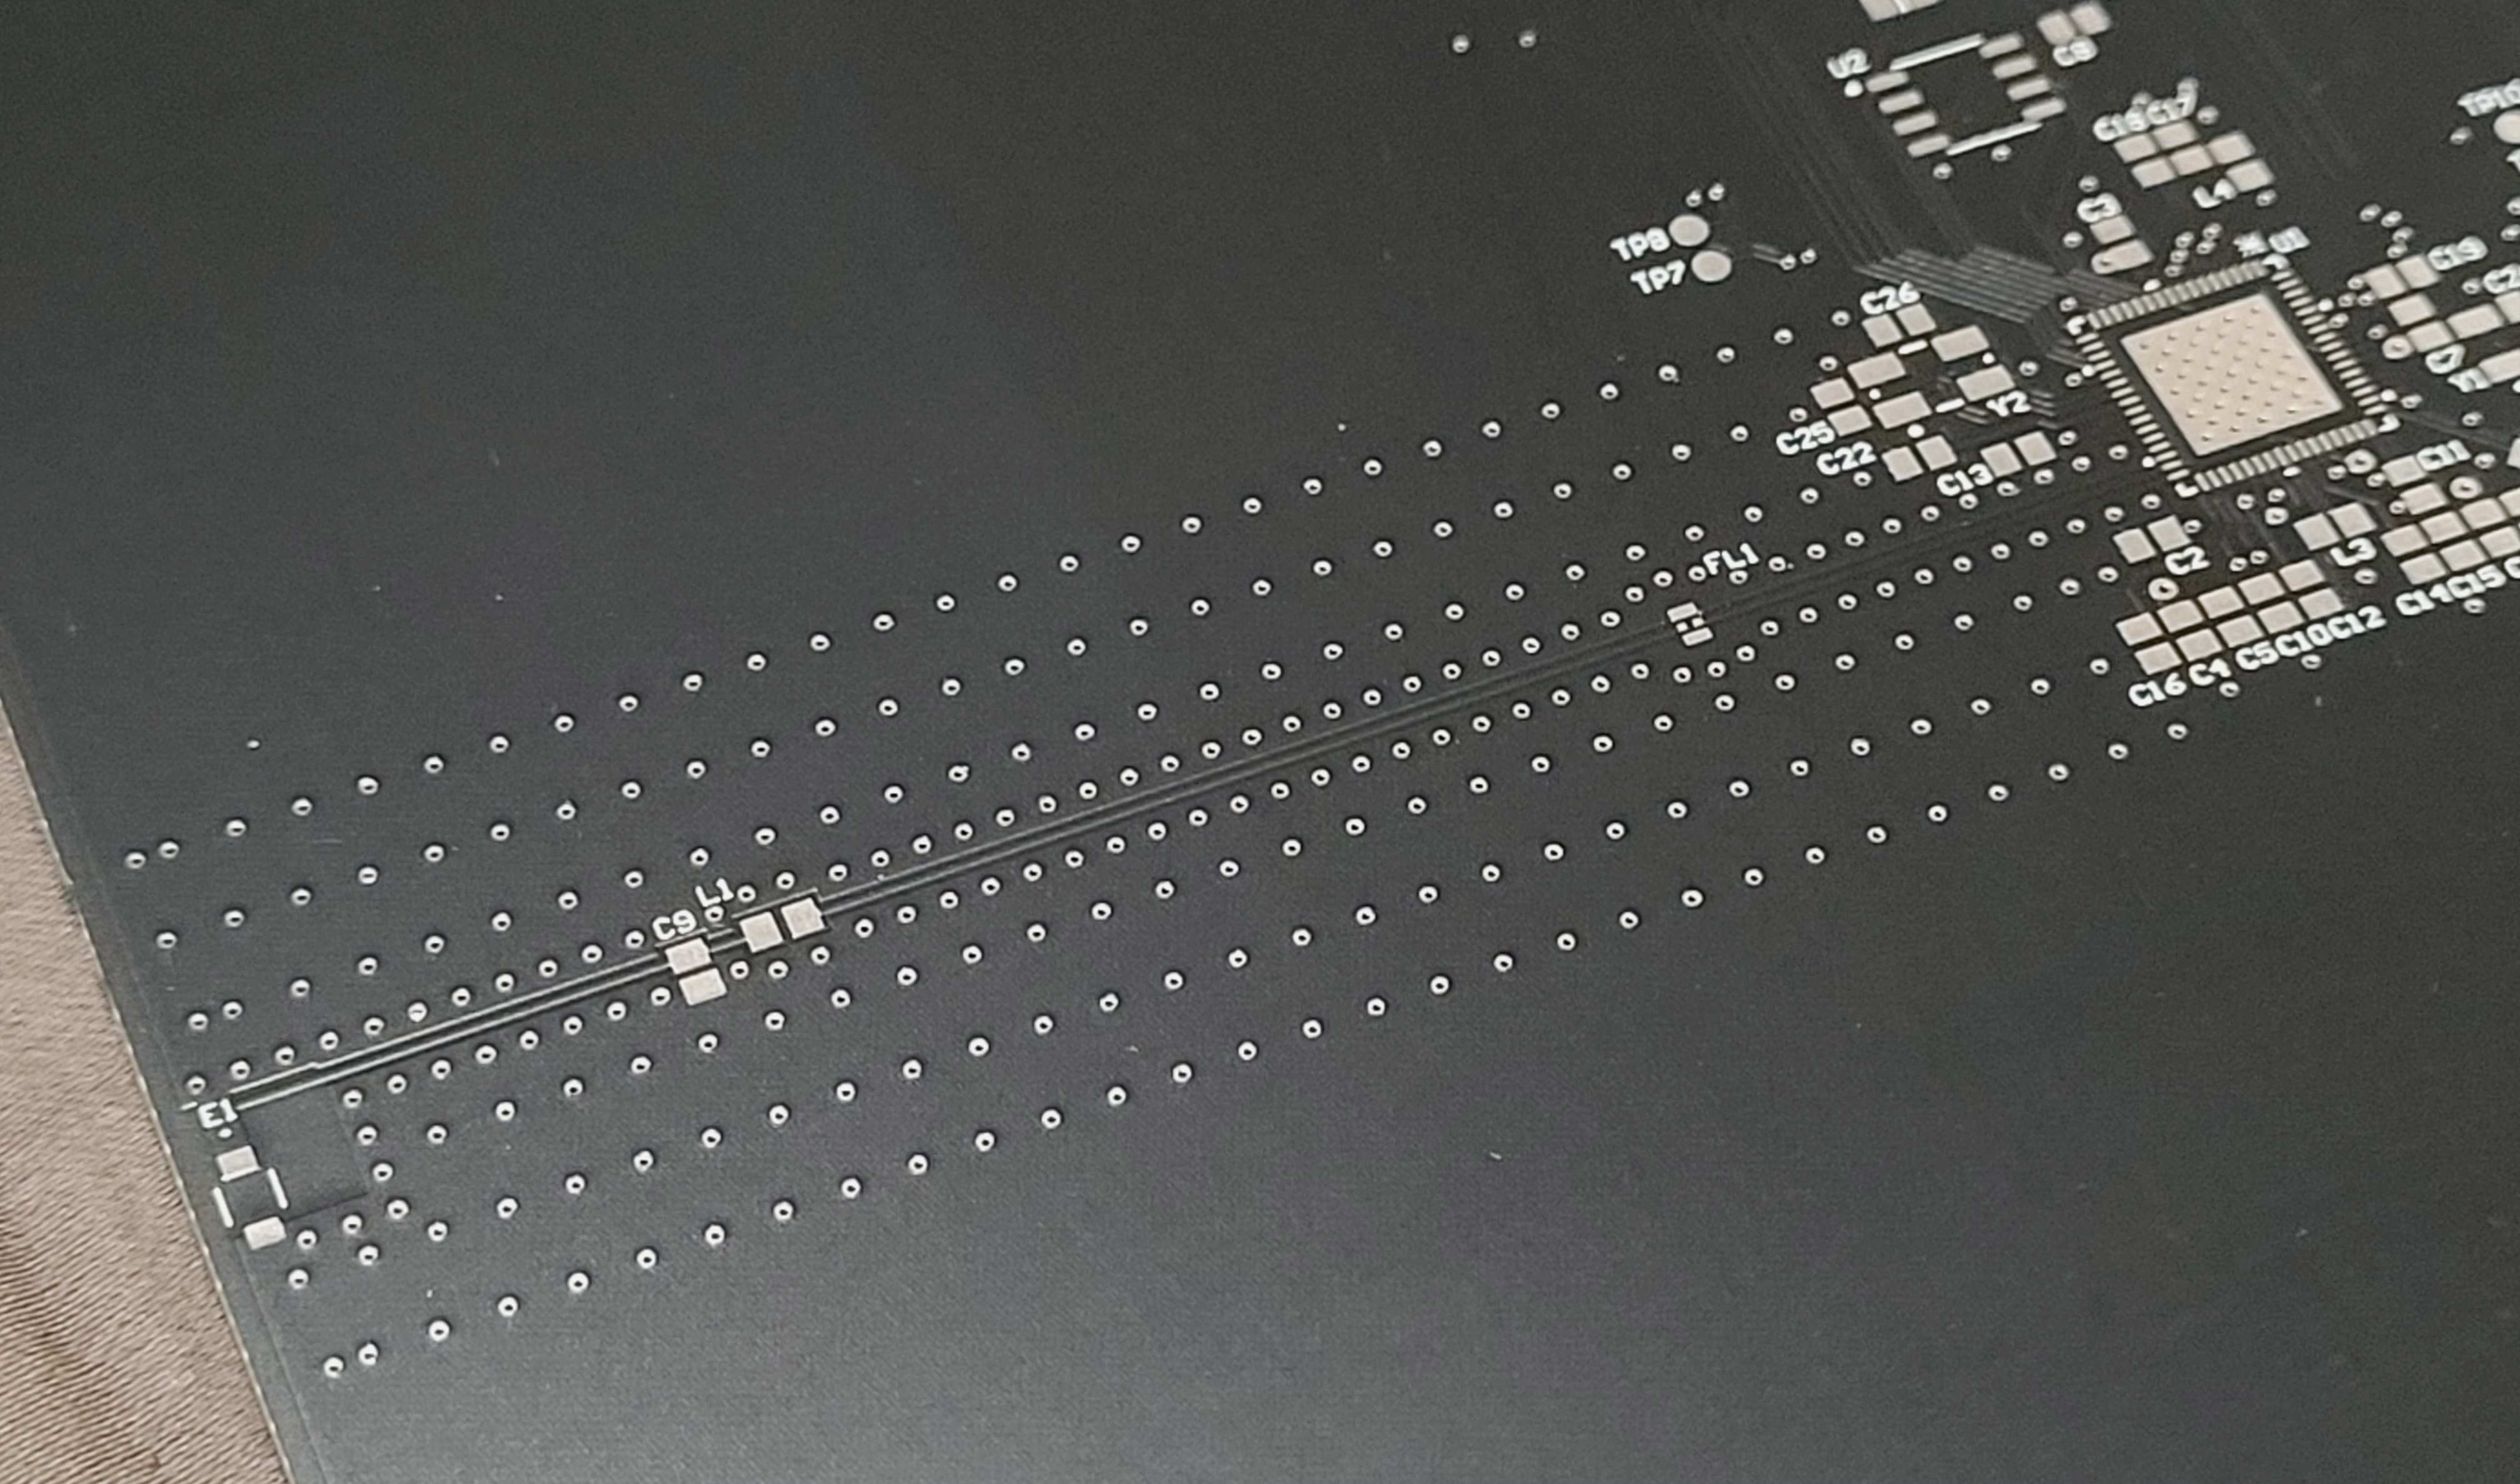
\includegraphics[width=\linewidth]{images/mcu_v1_cpwg.jpg}
    \caption{The coplanar waveguide designed to carry a 2.4 GHz signal surrounded by via fencing.}
\end{figure}